\documentclass[12pt,a4paper]{article}
\renewcommand{\thesection}{\Roman{section}}
\renewcommand{\thesubsection}{\thesection.\Roman{subsection}}
\usepackage{xeCJK}
\usepackage{caption}
\usepackage{amssymb}
\usepackage{amsmath}
\usepackage{geometry}
\usepackage{subfigure}
\usepackage{fancyhdr}
\usepackage[export]{adjustbox}
\usepackage{graphicx}
\graphicspath{{images/}}
\geometry{left=2.5cm,right=1.5cm,top=2cm,bottom=2cm}

\title{Deep Learning and Practice \\Lab6 \\ Report}
\date{May 23, 2019}
\author{呂紹篁, 0751904}
\setCJKmainfont{AR PL UKai CN}
\begin{document}
\captionsetup[figure]{labelfont={bf},labelformat={default},labelsep=period,name={Fig.}}
\thispagestyle{plain}
\cfoot{}
\maketitle

\section{Intoduction} \label{sec:intro}
Traditional GAN has the problem that when we change the specific dimension of noise consecutive, we cannot interpret the generative result since they don't have obvious relation. \textbf{InfoGAN}, try to split noise into two parts: latend part and pure noise part, if we change latend part consecutive, we can observe the relation between results, for example, the thickness or the rotation. In this lab, we try to use InfoGAN to generate a handwritten digits with MNIST dataset.

\begin{figure}[hbt]
\centering
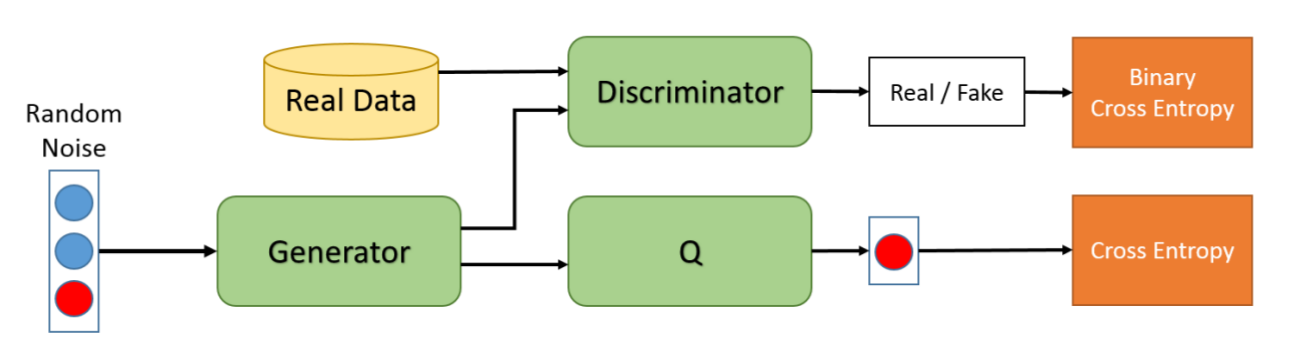
\includegraphics[scale=0.3]{infogan.png}
\caption{System of InfoGAN}
\label{fig:infogan}
\end{figure}

\section{Experiment Setups} \label{sec:exp_setup}
\subsection{Adversarial Loss}
To train a generative adversarial network, we have to maintain two networks, one for generator and other for discriminator. The discriminator review the real data from dataset and has the capability to identify whether the input is real or fake. The generator, on the other hand, try to use noise as input and generate an image, try to confuse the discriminator. The discriminator is simply a binary classifier, so we can use binary cross entropy as loss function. \\
From the PDF TA provided, the first generator loss make discriminator more powerful, i.e., it may occur that whatever what results generate from the generator, the disciminator always say they are fake, so we choose the second one. 
\subsection{Maximizing Mutual Information}
To make model learn the importance of latend code, we try to maximize the mutual information between latend code and its cooresponding generated output, this is what Q network trying to do.
\subsection{Generate Fixed Noise and Images}
We first generate 100 10-D one-hot vector, to make the same digit in the same column in the result, we generate this matrix with ten repeated 10-D identity. On the other hand, we sample 54-D from an uniform distribution, ranging from -1 to 1. Then, after the generator network trained, we concatenate this 10-D vector and 54-D noise to become a 64-D input and feed it into generator.
\subsection{Loss Function For Generator}
For the loss of generator, we use the second one, $ L_G =  E_\text{x$\sim$p}[-logD(x)]+L_I(G, Q)$


\section{Experimental Results} \label{sec:res}
\subsection{Samples}
\begin{figure}[hbt]
\centering
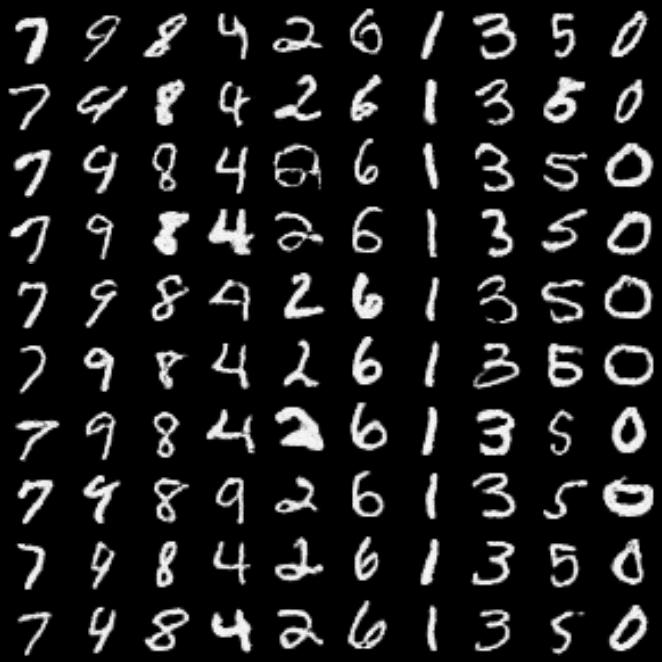
\includegraphics[scale=0.5]{sample.png}
\caption{100 Samples}
\label{fig:samples}
\end{figure}
From left to right: 7, 9, 8, 4, 2, 6, 1, 3, 5 and 0.
\subsection{Training Loss Curves}
\begin{figure}[hbt]
\centering
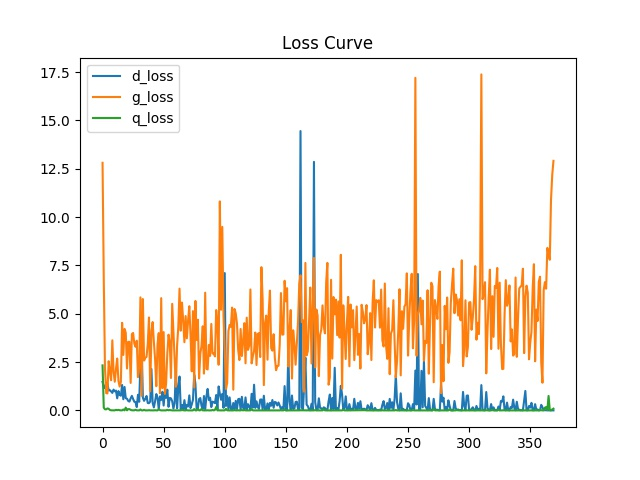
\includegraphics[scale=0.7]{loss.png}
\caption{Traing Loss Curve}
\label{fig:loss}
\end{figure}
\subsection{Probability Curves}
\begin{figure}[hbt]
\centering
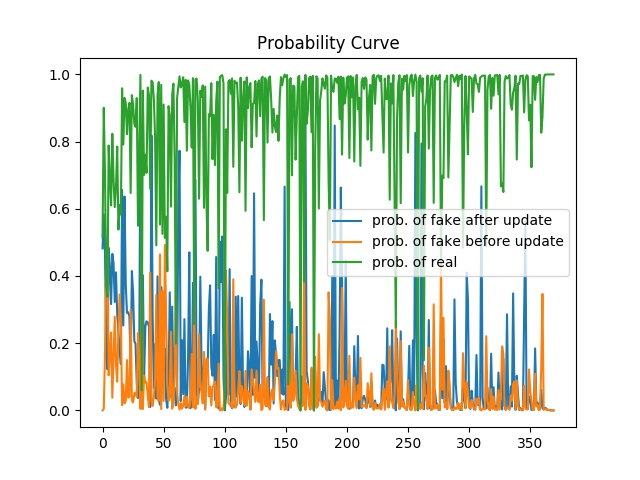
\includegraphics[scale=0.7]{prob.png}
\caption{Probability Curve}
\label{fig:prob}
\end{figure}

\section{Discussion} \label{sec:dis}
As the figures illustrated above, the probability vibrate seriously, this is not a good phenomenon. \\
Sometimes after serveral epochs, the generator suddenly "\textbf{broken}" and the loss of discriminator become extremely small. The phenomenon happened often and I have no idea why this occurred. \\
In this lab we only try the "hello world" of GAN, that is, handwritten digit generation, it will be interesting that we try different dataset and see the power of GAN.

%\bibliographystyle{IEEEtran}
%\bibliography{report.bib}

\end{document}
